% Capítulo 11: faixas de valores (partições) e fronteiras da função situacao(nota).
\documentclass[border=4pt]{standalone}
\usepackage[utf8]{inputenc}
\usepackage[T1]{fontenc}
% Estilo comum das figuras de vetores (capítulo 8).
\usepackage{tikz}
\usetikzlibrary{arrows.meta, positioning, calc, decorations.pathreplacing}
\definecolor{navy}{RGB}{23,45,80}
\definecolor{laranja}{RGB}{250,110,29}
\definecolor{cinzalogo}{RGB}{107,114,126}
\definecolor{azul}{RGB}{205,222,247}
\tikzset{
  casa/.style={draw=navy, line width=0.9pt, minimum width=8mm, minimum height=7mm,
               inner sep=0pt, font=\sffamily\small},
  pronta/.style={casa, fill=azul},
  parte/.style={casa, fill=laranja!12},
  marcada/.style={casa, fill=laranja!45, draw=laranja},
  fora/.style={casa, draw=cinzalogo!60, dashed, fill=white, text=cinzalogo!60},
  indice/.style={font=\sffamily\scriptsize, text=cinzalogo},
  explica/.style={font=\sffamily\small, text=navy, anchor=east},
  legenda/.style={font=\sffamily\scriptsize, text=cinzalogo},
  rotulo/.style={font=\sffamily\small\bfseries, text=navy},
  seta/.style={-{Stealth[length=2.2mm]}, navy, line width=0.9pt},
  chave/.style={decorate, decoration={brace, amplitude=4pt, mirror}, navy, line width=0.8pt},
}
% \vetor{nome}{x}{y}{valor/estilo, valor/estilo, ...}: casas lado a lado, chamadas nome0, nome1...
\newcommand{\vetor}[4]{%
  \foreach \valor/\estilo [count=\i from 0] in {#4} {
    \node[\estilo] (#1\i) at ($(#2, #3) + (\i*0.8, 0)$) {\valor};
  }
}

\tikzset{
  faixa/.style={draw=navy, line width=0.8pt, minimum height=8mm, font=\sffamily\small,
                inner sep=1pt, align=center},
  borda/.style={circle, fill=laranja, draw=laranja, inner sep=0pt, minimum size=2.2mm},
  valor/.style={font=\sffamily\scriptsize, text=laranja},
}
\begin{document}
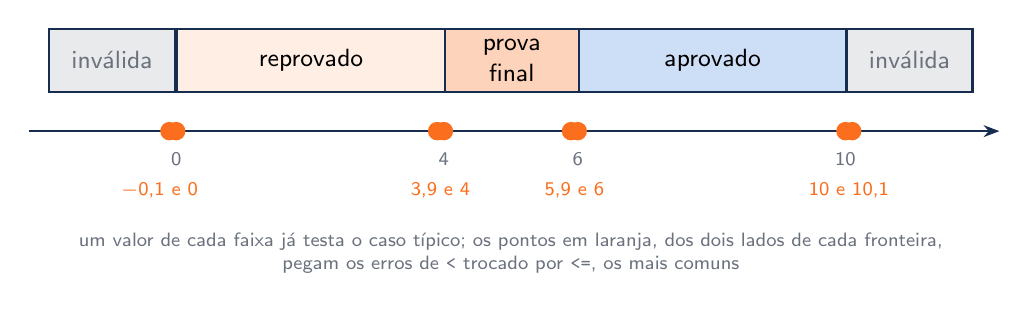
\begin{tikzpicture}[x=0.85cm]
  % faixas
  \node[faixa, fill=cinzalogo!15, text=cinzalogo, minimum width=1.6cm, anchor=east] at (0, 0) {inválida};
  \node[faixa, fill=laranja!12, minimum width=4*0.85cm, anchor=west] at (0, 0) {reprovado};
  \node[faixa, fill=laranja!30, minimum width=2*0.85cm, anchor=west] at (4, 0) {prova\\final};
  \node[faixa, fill=azul, minimum width=4*0.85cm, anchor=west] at (6, 0) {aprovado};
  \node[faixa, fill=cinzalogo!15, text=cinzalogo, minimum width=1.6cm, anchor=west] at (10, 0) {inválida};
  % eixo
  \draw[navy, line width=0.9pt, -{Stealth[length=2mm]}] (-2.2, -0.9) -- (12.3, -0.9);
  \foreach \x in {0, 4, 6, 10} {
    \draw[navy, line width=0.9pt] (\x, -0.8) -- (\x, -1.0);
    \node[indice] at (\x, -1.25) {\x};
  }
  % fronteiras testadas
  \foreach \x/\rotulo/\lado in {-0.1/-0{,}1/below, 0/0/above, 3.9/3{,}9/below, 4/4/above,
                                5.9/5{,}9/below, 6/6/above, 10/10/below, 10.1/10{,}1/above} {
    \node[borda] at (\x, -0.9) {};
  }
  \node[valor] at (-0.25, -1.65) {$-$0,1 e 0};
  \node[valor] at (3.95, -1.65) {3,9 e 4};
  \node[valor] at (5.95, -1.65) {5,9 e 6};
  \node[valor] at (10.05, -1.65) {10 e 10,1};
  \node[legenda, align=center] at (5, -2.45)
    {um valor de cada faixa já testa o caso típico; os pontos em laranja, dos dois lados de cada fronteira,\\
     pegam os erros de \texttt{<} trocado por \texttt{<=}, os mais comuns};
\end{tikzpicture}
\end{document}
